% !TeX program = xelatex
\documentclass[12pt,a4paper]{article}
\usepackage{fontspec}
\setmainfont{Times New Roman}[Path=C:/Windows/Fonts/,UprightFont=times.ttf,BoldFont=timesbd.ttf,ItalicFont=timesi.ttf,BoldItalicFont=timesbi.ttf]
\usepackage{amsmath,amssymb,amsfonts}
\usepackage[left=1.5cm,right=1.5cm,top=1.5cm,bottom=1.7cm,headheight=17pt]{geometry}
\usepackage{enumitem,array,graphicx,tikz,fancyhdr,needspace}
\usetikzlibrary{arrows.meta,calc,patterns}
% Sửa số đề và số trang đề thực tế sau khi biên dịch/tách PDF.
\newcommand{\soDe}{1}
\newcommand{\soTrangDe}{4}
\newcommand{\maDe}{\ifnum\soDe<1000 0\fi\ifnum\soDe<100 0\fi\ifnum\soDe<10 0\fi\soDe}
\pagestyle{fancy}
\fancyhf{}
\lhead{\small\textbf{ÔN TẬP GIỮA KÌ I}}
\rhead{\small\textit{Biên soạn: Dương Gia Bảo}}
\rfoot{\small Trang \thepage/\soTrangDe\ - Mã đề: \maDe}
\renewcommand{\headrulewidth}{0.4pt}
\fancypagestyle{answers}{\rfoot{\small Trang \thepage\ - Mã đề: \maDe}}
\fancypagestyle{firstpage}{\fancyhead{}\renewcommand{\headrulewidth}{0pt}}
\setlength{\parindent}{0pt}
\setlength{\parskip}{3pt}
\setlength{\emergencystretch}{1em}
\setlist[enumerate,1]{label=\textbf{Câu \arabic*:},leftmargin=*,itemsep=8pt,topsep=5pt}
\setlist[enumerate,2]{label=\alph*),leftmargin=*,itemsep=3pt,topsep=3pt}
\newcommand{\bonpa}[4]{\par\nobreak\smallskip\nobreak\noindent
\begin{tabular}{@{}p{0.47\linewidth}p{0.47\linewidth}@{}}
\textbf{A.} #1 & \textbf{B.} #2\\[8pt]
\textbf{C.} #3 & \textbf{D.} #4\end{tabular}}
\newcommand{\loigiai}[1]{\par\medskip\Needspace{4\baselineskip}\noindent\textbf{#1}\par\nobreak}
\newcommand{\otraloi}{\par\nobreak\smallskip\noindent\textit{Trả lời:}\quad\fbox{\rule{0pt}{11pt}\makebox[0.3cm]{}}\,\fbox{\rule{0pt}{11pt}\makebox[0.3cm]{}}\,\fbox{\rule{0pt}{11pt}\makebox[0.3cm]{}}\,\fbox{\rule{0pt}{11pt}\makebox[0.3cm]{}}}
\begin{document}
\thispagestyle{firstpage}
\noindent
\begin{minipage}[t]{0.35\textwidth}
    \centering
    {\fontsize{13}{15}\selectfont\textbf{ÔN TẬP GIỮA KÌ I}}\\[5pt]
    \textit{Biên soạn: Dương Gia Bảo}\\[6pt]
    \setlength{\fboxrule}{0.8pt}%
    \setlength{\fboxsep}{5pt}%
    \fbox{\begin{minipage}{0.83\linewidth}
        \centering
        {\fontsize{13}{15}\selectfont\textbf{ĐỀ ÔN TẬP}\\[2pt]\textbf{CHƯƠNG I VÀ II}}\\[5pt]
        \textit{(Đề thi gồm có \ifnum\soTrangDe<10 0\fi\soTrangDe\ trang)}
    \end{minipage}}
\end{minipage}\hfill
\begin{minipage}[t]{0.63\textwidth}
    \centering
    {\fontsize{13}{15}\selectfont\textbf{ÔN TẬP KIỂM TRA GIỮA KÌ I}\\[2pt]
    \textbf{NĂM HỌC 2026 - 2027}}\\[6pt]
    {\fontsize{14}{16}\selectfont\textbf{Môn: TOÁN - Lớp 12 (ĐỀ SỐ \soDe)}}\\[5pt]
    {\fontsize{11.5}{13}\selectfont\textit{Thời gian làm bài: 90 phút, không kể thời gian giao đề}}\\[6pt]
    \setlength{\fboxrule}{0.8pt}%
    \setlength{\fboxsep}{6pt}%
    \fbox{\makebox[3cm]{\fontsize{14}{16}\selectfont\textbf{Mã đề: \maDe}}}
\end{minipage}
\par\vspace{3pt}
\hrule height 0.6pt
\vspace{4pt}
\noindent\textit{Họ và tên học sinh:}\dotfill\hspace{1cm}\textit{Lớp:}\makebox[3.5cm]{\dotfill}
\par\vspace{3pt}
\hrule height 0.6pt
\vspace{4pt}


\vspace{3pt}
\section*{\large PHẦN I. Câu trắc nghiệm nhiều phương án lựa chọn}
\textit{Thí sinh trả lời từ câu 1 đến câu 12. Mỗi câu chỉ chọn một phương án.}
\begin{enumerate}
\item Cho hàm số $y=x^3-3x^2+2$. Hàm số nghịch biến trên khoảng nào sau đây?
\bonpa{$(0;2)$.}{$(-\infty;0)$.}{$(2;+\infty)$.}{$(-\infty;+\infty)$.}

\item Điểm cực đại của đồ thị hàm số $y=-x^3+3x+1$ là
\bonpa{$(-1;-1)$.}{$(1;1)$.}{$(1;3)$.}{$(-1;3)$.}

\item Giá trị lớn nhất của hàm số $f(x)=x^3-3x$ trên đoạn $[-2;1]$ bằng
\bonpa{$0$.}{$2$.}{$-2$.}{$4$.}

\item Các tiệm cận đứng và tiệm cận ngang của đồ thị $y=\dfrac{2x-1}{x+3}$ lần lượt là
\bonpa{$x=3$ và $y=2$.}{$x=-3$ và $y=-2$.}{$x=2$ và $y=-3$.}{$x=-3$ và $y=2$.}

\item Đường tiệm cận xiên của đồ thị hàm số $y=\dfrac{x^2+1}{x-1}$ có phương trình là
\bonpa{$y=x+1$.}{$y=x-1$.}{$y=2x+1$.}{$y=1$.}

\Needspace{7\baselineskip}
\item Đường cong trong hình bên là đồ thị của hàm số nào dưới đây?
\par\nobreak\smallskip
\begin{minipage}[c]{0.60\linewidth}
\bonpa{$y=-x^3+3x$.}{$y=x^3-3x$.}{$y=x^3+3x$.}{$y=x^3-3x+1$.}
\end{minipage}\hfill
\begin{minipage}[c]{0.36\linewidth}\centering
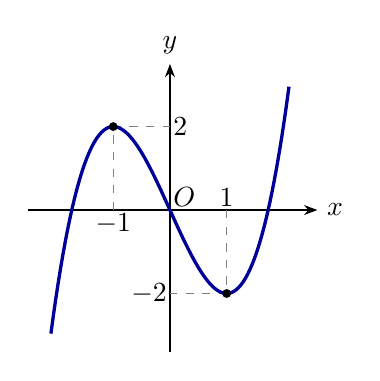
\begin{tikzpicture}[x=0.72cm,y=0.53cm,>=Stealth]
\draw[->] (-2.5,0)--(2.6,0) node[right] {$x$};
\draw[->] (0,-3.4)--(0,3.5) node[above] {$y$};
\draw[dashed,gray] (-1,0)--(-1,2)--(0,2);
\draw[dashed,gray] (1,0)--(1,-2)--(0,-2);
\draw[very thick,blue!60!black,domain=-2.1:2.1,samples=100] plot (\x,{\x*\x*\x-3*\x});
\fill (-1,2) circle (1.6pt);\fill (1,-2) circle (1.6pt);
\node[above right,fill=white,inner sep=1pt] at (0,0) {$O$};
\node[below,fill=white,inner sep=1pt] at (-1,0) {$-1$};
\node[above,fill=white,inner sep=1pt] at (1,0) {$1$};
\node[right,fill=white,inner sep=1pt] at (0,2) {$2$};
\node[left,fill=white,inner sep=1pt] at (0,-2) {$-2$};
\end{tikzpicture}
\end{minipage}

\item Theo một mô hình, nồng độ của một chất trong bể sau $t$ giờ là
$c(t)=-t^3+6t^2+15$ (mg/L), với $0\le t\le5$. Nồng độ đạt giá trị lớn nhất tại thời điểm nào?
\bonpa{$t=1$ giờ.}{$t=2$ giờ.}{$t=3$ giờ.}{$t=4$ giờ.}
\end{enumerate}

\begin{enumerate}[start=8]
\item Cho tứ diện $ABCD$. Vectơ $\overrightarrow{AB}+\overrightarrow{BC}+\overrightarrow{CD}$ bằng
\bonpa{$\overrightarrow{AC}$.}{$\overrightarrow{BD}$.}{$\overrightarrow{AD}$.}{$\overrightarrow{DA}$.}

\item Trong không gian $Oxyz$, cho $A(1;-2;3)$ và $B(4;0;-1)$. Tọa độ của $\overrightarrow{AB}$ là
\bonpa{$(5;-2;2)$.}{$(3;2;-4)$.}{$(-3;-2;4)$.}{$(3;-2;-4)$.}

\item Cho $\vec a=(2;-1;3)$ và $\vec b=(1;2;-1)$. Tích vô hướng $\vec a\cdot\vec b$ bằng
\bonpa{$3$.}{$0$.}{$-1$.}{$-3$.}

\item Trong không gian $Oxyz$, độ dài của vectơ $\vec u=(1;2;-2)$ bằng
\bonpa{$\sqrt5$.}{$5$.}{$3$.}{$9$.}

\item Trong không gian $Oxyz$, cho $A(0;2;1)$ và $B(4;-2;3)$. Trung điểm của $AB$ có tọa độ là
\bonpa{$(2;0;2)$.}{$(4;0;4)$.}{$(2;-2;1)$.}{$(-2;2;-1)$.}
\end{enumerate}

\section*{\large PHẦN II. Câu trắc nghiệm đúng hoặc sai}
\textit{Thí sinh trả lời từ câu 1 đến câu 4. Trong mỗi ý a), b), c), d), chọn đúng hoặc sai.}
\begin{enumerate}
\Needspace{9\baselineskip}
\item Cho hàm số $f(x)=\dfrac{x^2-2x+2}{x-1}$, xác định trên $\mathbb R\setminus\{1\}$.
\begin{enumerate}
\item $f'(x)=\dfrac{x(x-2)}{(x-1)^2}$.
\item Hàm số đồng biến trên khoảng $(0;1)$.
\item Đồ thị hàm số có tiệm cận xiên là đường thẳng $y=x-1$.
\item Khoảng cách giữa hai điểm cực trị của đồ thị hàm số bằng $2\sqrt2$.
\end{enumerate}

\Needspace{10\baselineskip}
\item Một cơ sở sản xuất và bán hết $x$ sản phẩm mỗi ngày, với $x$ là số nguyên và $0\le x\le200$.
Giá bán mỗi sản phẩm là $p(x)=500-2x$ (nghìn đồng). Tổng chi phí trong ngày là
$C(x)=100x+6000$ (nghìn đồng).
\begin{enumerate}
\item Doanh thu trong ngày là $R(x)=-2x^2+500x$ (nghìn đồng).
\item Lợi nhuận trong ngày là $P(x)=-2x^2+400x-6000$ (nghìn đồng).
\item Lợi nhuận lớn nhất đạt được khi bán $125$ sản phẩm trong ngày.
\item Khi chọn giá bán $300$ nghìn đồng một sản phẩm, cơ sở đạt lợi nhuận lớn nhất là $14$ triệu đồng mỗi ngày.
\end{enumerate}
\end{enumerate}

\begin{enumerate}[start=3]
\item Trong không gian $Oxyz$, cho ba điểm $A(1;0;2)$, $B(3;2;0)$ và $C(-1;2;4)$.
\begin{enumerate}
\item $\overrightarrow{AB}=(2;2;-2)$.
\item Trọng tâm của tam giác $ABC$ là điểm $G(1;2;2)$.
\item Hai vectơ $\overrightarrow{AB}$ và $\overrightarrow{AC}$ vuông góc với nhau.
\item Điểm $D(-3;0;6)$ là đỉnh còn lại để $ABCD$ là hình bình hành theo thứ tự các đỉnh $A,B,C,D$.
\end{enumerate}

\item Một biển hiệu được giữ bởi hai dây. Trong hệ tọa độ $Oxyz$, hai lực căng dây tác dụng lên
biển hiệu được mô hình hóa bởi $\vec F_1=(30;0;40)$ và $\vec F_2=(-30;0;40)$, đơn vị newton (N).
Một vật cân bằng khi tổng các vectơ lực tác dụng lên vật bằng $\vec0$.
\begin{enumerate}
\item $\vec F_1+\vec F_2=\vec0$.
\item Độ lớn của lực $\vec F_1$ bằng $50$ N.
\item $\vec F_1\cdot\vec F_2=700$.
\item Nếu biển hiệu chỉ chịu hai lực căng trên và trọng lực $\vec P=(0;0;-80)$ thì biển hiệu cân bằng.
\end{enumerate}
\end{enumerate}

\section*{\large PHẦN III. Câu trắc nghiệm trả lời ngắn}
\textit{Thí sinh trả lời từ câu 1 đến câu 6. Ghi kết quả vào các ô trả lời; dùng dấu phẩy cho phần thập phân.}
\begin{enumerate}
\item Có bao nhiêu giá trị nguyên của $m$ thuộc đoạn $[-7;7]$ để hàm số
$y=\dfrac{x+m}{x-2}$ đồng biến trên từng khoảng xác định của nó?
\otraloi

\item Trong không gian $Oxyz$, cho hình hộp $ABCD.A'B'C'D'$ có
$A(1;1;0)$, $B(3;1;1)$, $D(0;3;1)$ và $A'(2;0;4)$.
Biết $C'(a;b;c)$, tính $a+b+c$.
\otraloi
\end{enumerate}

\newpage
\begin{enumerate}[start=3]
\item Từ một tấm bìa hình chữ nhật kích thước $40$ cm $\times$ $25$ cm, người ta cắt ở bốn góc
bốn hình vuông bằng nhau, mỗi hình có cạnh $x$ cm, rồi gấp phần còn lại thành một chiếc hộp không nắp.
Bỏ qua độ dày tấm bìa. Thể tích lớn nhất của chiếc hộp bằng bao nhiêu cm$^3$?
\begin{center}
\begin{tikzpicture}[x=0.13cm,y=0.13cm,>=Stealth]
\fill[pattern=north east lines,pattern color=gray] (0,0) rectangle (5,5);
\fill[pattern=north east lines,pattern color=gray] (35,0) rectangle (40,5);
\fill[pattern=north east lines,pattern color=gray] (0,20) rectangle (5,25);
\fill[pattern=north east lines,pattern color=gray] (35,20) rectangle (40,25);
\draw[thick] (0,0) rectangle (40,25);
\draw[dashed] (5,0)--(5,25) (35,0)--(35,25) (0,5)--(40,5) (0,20)--(40,20);
\draw[<->] (0,-3)--(40,-3) node[midway,fill=white,inner sep=1pt] {$40$ cm};
\draw[<->] (44,0)--(44,25) node[midway,right] {$25$ cm};
\draw[<->] (0,28)--(5,28) node[midway,above] {$x$};
\node[font=\small] at (20,12.5) {Phần bìa giữ lại};
\end{tikzpicture}
\par\smallskip{\small\textit{Hình minh họa, không theo tỉ lệ.}}
\end{center}
\otraloi

\item Trong không gian $Oxyz$ với đơn vị mét, hai thiết bị bay có vị trí sau $t$ giây lần lượt là
$A_t(3t;t;2)$ và $B_t(12-t;4+t;8)$, với $0\le t\le5$.
Khoảng cách nhỏ nhất giữa hai thiết bị trong khoảng thời gian này bằng bao nhiêu mét?
\textit{Làm tròn kết quả đến hàng phần mười.}
\otraloi

\item Cho hàm số $y=x^3-3mx+2$ với $m>0$. Đồ thị có hai điểm cực trị $A$ và $B$.
Tìm $m$ để $AB=2\sqrt{34}$.
\otraloi

\item Một trạm điện $A$ nằm trên bờ biển thẳng. Điểm $B$ trên đảo cách bờ $3$ km;
gọi $C$ là chân đường vuông góc từ $B$ xuống bờ, biết $AC=8$ km.
Người ta kéo cáp từ $A$ dọc bờ đến một điểm $D$ trên đoạn $AC$, rồi kéo thẳng từ $D$ đến $B$.
Chi phí cáp trên bờ là $60$ triệu đồng/km và dưới biển là $100$ triệu đồng/km.
Chi phí thấp nhất của tuyến cáp bằng bao nhiêu triệu đồng?
\otraloi
\end{enumerate}
\begin{center}\textbf{---------------- HẾT ----------------}\end{center}

\newpage\pagestyle{answers}
\begin{center}\Large\textbf{BẢNG ĐÁP ÁN TỔNG HỢP}\end{center}
\textbf{Phần I. Trắc nghiệm nhiều phương án lựa chọn}
\begin{center}
\renewcommand{\arraystretch}{1.5}
\begin{tabular}{|c|*{12}{c|}}\hline
Câu & 1&2&3&4&5&6&7&8&9&10&11&12\\\hline
Đáp án & A & C & B & D & A & B & D & C & B & D & C & A \\\hline
\end{tabular}
\end{center}

\textbf{Phần II. Đúng hoặc sai}
\begin{center}
\renewcommand{\arraystretch}{1.4}
\begin{tabular}{|c|c|c|c|c|}\hline
Câu & a) & b) & c) & d)\\\hline
1 & Đ & S & Đ & S\\\hline
2 & Đ & Đ & S & Đ\\\hline
3 & Đ & S & S & Đ\\\hline
4 & S & Đ & Đ & Đ\\\hline
\end{tabular}
\end{center}

\textbf{Phần III. Trả lời ngắn}
\begin{center}
\renewcommand{\arraystretch}{1.5}
\begin{tabular}{|c|c|c|c|c|c|c|}\hline
Câu & 1 & 2 & 3 & 4 & 5 & 6\\\hline
Đáp án & 5 & 11 & 2250 & 7,2 & 2 & 720 \\\hline
\end{tabular}
\end{center}

\textbf{Thang điểm dùng cho đề ôn tập:}
\begin{itemize}[leftmargin=*,itemsep=3pt]
\item Phần I: mỗi câu đúng $0{,}25$ điểm; tối đa $3$ điểm.
\item Phần II: mỗi câu có 4 ý. Đúng 1, 2, 3, 4 ý lần lượt được $0{,}1$; $0{,}25$; $0{,}5$; $1$ điểm. Tối đa $4$ điểm.
\item Phần III: mỗi câu đúng $0{,}5$ điểm; tối đa $3$ điểm.
\end{itemize}
\textbf{Phạm vi:} Bài 1–5 (ứng dụng đạo hàm và khảo sát hàm số), Bài 6–8 (vectơ và tọa độ trong không gian).
Tổng điểm $10$; thời gian $90$ phút.

\newpage
\begin{center}\Large\textbf{HƯỚNG DẪN GIẢI CHI TIẾT}\end{center}
\section*{\large Phần I}
\loigiai{Câu 1. Chọn A.}
Ta có $y'=3x^2-6x=3x(x-2)$. Đạo hàm âm khi $0<x<2$, nên hàm số nghịch biến trên $(0;2)$.

\loigiai{Câu 2. Chọn C.}
$y'=3-3x^2=0\Leftrightarrow x=\pm1$. Khi qua $x=1$, đạo hàm đổi dấu từ dương sang âm, nên hàm số đạt cực đại tại $x=1$. Vì $y(1)=3$, điểm cực đại của đồ thị là $(1;3)$.

\loigiai{Câu 3. Chọn B.}
$f'(x)=3x^2-3=0\Leftrightarrow x=\pm1$. Xét trên $[-2;1]$, ta tính
$f(-2)=-2$, $f(-1)=2$, $f(1)=-2$. Do đó giá trị lớn nhất bằng $2$.

\loigiai{Câu 4. Chọn D.}
Tại $x=-3$, mẫu số bằng $0$ còn tử số bằng $-7\ne0$, nên $x=-3$ là tiệm cận đứng.
Mặt khác, $\lim_{x\to\pm\infty}\dfrac{2x-1}{x+3}=2$, nên $y=2$ là tiệm cận ngang.

\loigiai{Câu 5. Chọn A.}
Chia đa thức: $\dfrac{x^2+1}{x-1}=x+1+\dfrac2{x-1}$. Vì $\dfrac2{x-1}\to0$ khi $x\to\pm\infty$, tiệm cận xiên là $y=x+1$.

\loigiai{Câu 6. Chọn B.}
Đồ thị đi qua gốc tọa độ, có cực đại tại hoành độ $-1$ với tung độ $2$, cực tiểu tại hoành độ $1$ với tung độ $-2$, và nhánh phải hướng lên.
Hàm $y=x^3-3x$ có $y'=3(x^2-1)$ và đúng các đặc điểm trên. Phương án A có hướng hai nhánh ngược lại; C luôn đồng biến; D không đi qua gốc tọa độ.

\loigiai{Câu 7. Chọn D.}
$c'(t)=-3t^2+12t=3t(4-t)$. Trên $[0;5]$, hàm tăng đến $t=4$ rồi giảm.
Ngoài ra, $c(0)=15$, $c(4)=47$, $c(5)=40$. Nồng độ đạt giá trị lớn nhất tại $t=4$ giờ.

\loigiai{Câu 8. Chọn C.}
Theo quy tắc ba điểm, $\overrightarrow{AB}+\overrightarrow{BC}=\overrightarrow{AC}$ và
$\overrightarrow{AC}+\overrightarrow{CD}=\overrightarrow{AD}$.

\loigiai{Câu 9. Chọn B.}
$\overrightarrow{AB}=(4-1;0-(-2);-1-3)=(3;2;-4)$.

\loigiai{Câu 10. Chọn D.}
$\vec a\cdot\vec b=2\cdot1+(-1)\cdot2+3\cdot(-1)=-3$.

\loigiai{Câu 11. Chọn C.}
$|\vec u|=\sqrt{1^2+2^2+(-2)^2}=\sqrt9=3$.

\loigiai{Câu 12. Chọn A.}
Trung điểm có tọa độ $\left(\dfrac{0+4}2;\dfrac{2+(-2)}2;\dfrac{1+3}2\right)=(2;0;2)$.

\newpage
\section*{\large Phần II}
\loigiai{Câu 1. a) Đúng; b) Sai; c) Đúng; d) Sai.}
Viết $f(x)=x-1+\dfrac1{x-1}$, suy ra
\[
f'(x)=1-\frac1{(x-1)^2}=\frac{x(x-2)}{(x-1)^2}.
\]
\begin{enumerate}[label=\alph*),leftmargin=*,itemsep=4pt]
\item Công thức đạo hàm đã cho đúng với mọi $x\ne1$.
\item Với $0<x<1$, tử số $x(x-2)<0$ và mẫu số dương, nên $f'(x)<0$. Hàm số nghịch biến trên $(0;1)$.
\item $f(x)-(x-1)=\dfrac1{x-1}\to0$ khi $x\to\pm\infty$, nên $y=x-1$ là tiệm cận xiên.
\item $f'(x)=0$ tại $x=0,2$; đạo hàm đổi dấu tại cả hai điểm. Hai điểm cực trị là $M(0;-2)$ và $N(2;2)$.
Do đó $MN=\sqrt{(2-0)^2+(2-(-2))^2}=\sqrt{20}=2\sqrt5$, khác $2\sqrt2$.
\end{enumerate}

\loigiai{Câu 2. a) Đúng; b) Đúng; c) Sai; d) Đúng.}
\begin{enumerate}[label=\alph*),leftmargin=*,itemsep=4pt]
\item Doanh thu bằng số lượng nhân giá bán: $R(x)=x(500-2x)=-2x^2+500x$.
\item Lợi nhuận bằng doanh thu trừ tổng chi phí:
\[
P(x)=R(x)-C(x)=-2x^2+400x-6000=-2(x-100)^2+14000.
\]
\item Với $0\le x\le200$, lợi nhuận lớn nhất khi $x=100$. Giá trị này là số nguyên nên thỏa điều kiện sản lượng. Tại $x=125$, lợi nhuận chỉ là $12750$ nghìn đồng.
\item Khi $x=100$, giá bán $p(100)=300$ nghìn đồng và lợi nhuận $P(100)=14000$ nghìn đồng, tức $14$ triệu đồng.
\end{enumerate}

\loigiai{Câu 3. a) Đúng; b) Sai; c) Sai; d) Đúng.}
\begin{enumerate}[label=\alph*),leftmargin=*,itemsep=4pt]
\item $\overrightarrow{AB}=B-A=(2;2;-2)$.
\item Trọng tâm là $G\left(\dfrac{1+3-1}3;\dfrac{0+2+2}3;\dfrac{2+0+4}3\right)=\left(1;\dfrac43;2\right)$.
\item $\overrightarrow{AC}=(-2;2;2)$ nên
$\overrightarrow{AB}\cdot\overrightarrow{AC}=-4+4-4=-4\ne0$. Hai vectơ không vuông góc.
\item Đỉnh thứ tư của hình bình hành thỏa $D=A+C-B=(-3;0;6)$.
\end{enumerate}

\loigiai{Câu 4. a) Sai; b) Đúng; c) Đúng; d) Đúng.}
\begin{enumerate}[label=\alph*),leftmargin=*,itemsep=4pt]
\item $\vec F_1+\vec F_2=(0;0;80)\ne\vec0$.
\item $|\vec F_1|=\sqrt{30^2+0^2+40^2}=50$ N.
\item $\vec F_1\cdot\vec F_2=30\cdot(-30)+0\cdot0+40\cdot40=700$.
\item $\vec F_1+\vec F_2+\vec P=(0;0;80)+(0;0;-80)=\vec0$. Theo điều kiện cân bằng trong đề, biển hiệu cân bằng.
\end{enumerate}

\newpage
\section*{\large Phần III}
\loigiai{Câu 1. Đáp án: 5.}
Tập xác định là $\mathbb R\setminus\{2\}$. Ta có
\[
y'=\frac{(x-2)-(x+m)}{(x-2)^2}=\frac{-m-2}{(x-2)^2}.
\]
Mẫu số dương trên từng khoảng xác định. Hàm số đồng biến trên cả hai khoảng khi $-m-2>0$, tức $m<-2$.
Nếu $m=-2$, hàm số bằng hằng số $1$ trên tập xác định nên không đồng biến.
Các giá trị nguyên cần tìm là $-7,-6,-5,-4,-3$, gồm $5$ giá trị.

\loigiai{Câu 2. Đáp án: 11.}
Quy tắc hình hộp cho
$\overrightarrow{AC'}=\overrightarrow{AB}+\overrightarrow{AD}+\overrightarrow{AA'}$.
Ta có
\[
\overrightarrow{AB}=(2;0;1),\quad
\overrightarrow{AD}=(-1;2;1),\quad
\overrightarrow{AA'}=(1;-1;4).
\]
Suy ra $\overrightarrow{AC'}=(2;1;6)$ và $C'=(1;1;0)+(2;1;6)=(3;2;6)$.
Vậy $a+b+c=3+2+6=11$.

\loigiai{Câu 3. Đáp án: 2250.}
Điều kiện để tạo được hộp là $0<x<12{,}5$. Chiều cao hộp là $x$, hai cạnh đáy là $40-2x$ và $25-2x$.
Thể tích:
\[
V(x)=x(40-2x)(25-2x)=4x^3-130x^2+1000x.
\]
Đạo hàm $V'(x)=12x^2-260x+1000=4(x-5)(3x-50)$.
Trong khoảng $(0;12{,}5)$, chỉ có nghiệm $x=5$ của $V'(x)=0$.
Đạo hàm dương trên $(0;5)$ và âm trên $(5;12{,}5)$, nên thể tích lớn nhất tại $x=5$.
Khi đó $V_{\max}=5\cdot30\cdot15=2250$ cm$^3$.

\loigiai{Câu 4. Đáp án: 7,2.}
Tại cùng thời điểm $t$, vectơ nối hai thiết bị là
$\overrightarrow{A_tB_t}=(12-4t;4;6)$.
Do đó
\[
A_tB_t^2=(12-4t)^2+4^2+6^2=16(t-3)^2+52\ge52.
\]
Dấu bằng xảy ra tại $t=3\in[0;5]$. Vì khoảng cách không âm,
$d_{\min}=\sqrt{52}=2\sqrt{13}\approx7{,}2111$ m. Làm tròn đến hàng phần mười được $7{,}2$ m.

\newpage
\loigiai{Câu 5. Đáp án: 2.}
$y'=3x^2-3m=0\Leftrightarrow x=\pm\sqrt m$ vì $m>0$.
Hai điểm cực trị có tọa độ
\[
A(-\sqrt m;2+2m\sqrt m),\qquad B(\sqrt m;2-2m\sqrt m).
\]
Suy ra $AB^2=(2\sqrt m)^2+(4m\sqrt m)^2=4m+16m^3$.
Theo đề bài, $AB^2=(2\sqrt{34})^2=136$, nên
\[
4m^3+m-34=0
\ \Longleftrightarrow\ (m-2)(4m^2+8m+17)=0.
\]
Vì $4m^2+8m+17=4(m+1)^2+13>0$, phương trình có nghiệm duy nhất $m=2$, thỏa điều kiện.

\loigiai{Câu 6. Đáp án: 720.}
Đặt $CD=x$ (km), $0\le x\le8$. Vì $D$ thuộc đoạn $AC$, ta có $AD=8-x$.
Tam giác $DCB$ vuông tại $C$, nên $DB=\sqrt{x^2+9}$.
Tổng chi phí, tính theo triệu đồng, là
\[
T(x)=60(8-x)+100\sqrt{x^2+9}.
\]
Đạo hàm:
\[
T'(x)=-60+\frac{100x}{\sqrt{x^2+9}}.
\]
Giải $T'(x)=0$ trên $[0;8]$:
\[
\frac{x}{\sqrt{x^2+9}}=\frac35
\ \Longleftrightarrow\ 25x^2=9(x^2+9)
\ \Longleftrightarrow\ x=\frac94.
\]
Với $x\ge0$, nghiệm thỏa mãn phương trình gốc là $x=\dfrac94$. Hơn nữa,
$T''(x)=\dfrac{900}{(x^2+9)^{3/2}}>0$, nên $T'$ tăng và đổi dấu từ âm sang dương tại $x=\dfrac94$.
Chi phí thấp nhất là
\[
T\!\left(\frac94\right)=60\cdot\frac{23}4+100\cdot\frac{15}4=345+375=720\text{ triệu đồng}.
\]

\end{document}
